\section{LINUX软硬件系统观察与分析}
\subsection{计算机硬件详细信息(3分)}
\begin{enumerate}
	\item CPU个数:\dlmu[3cm]{1}
	\item CPU物理核数:\dlmu[3cm]{1}
	\item CPU逻辑处理器个数:\dlmu[3cm]{1}
	\item MEM\ Total:\dlmu[3cm]{4026824}  
	\item MEM\ Used:\dlmu[3cm]{2959856}    
	\item MEM\ Swap:\dlmu[3cm]{4192252}  
\end{enumerate}

\begin{figure}[H]
	\begin{minipage}[c]{0.5\linewidth}
		\centering
		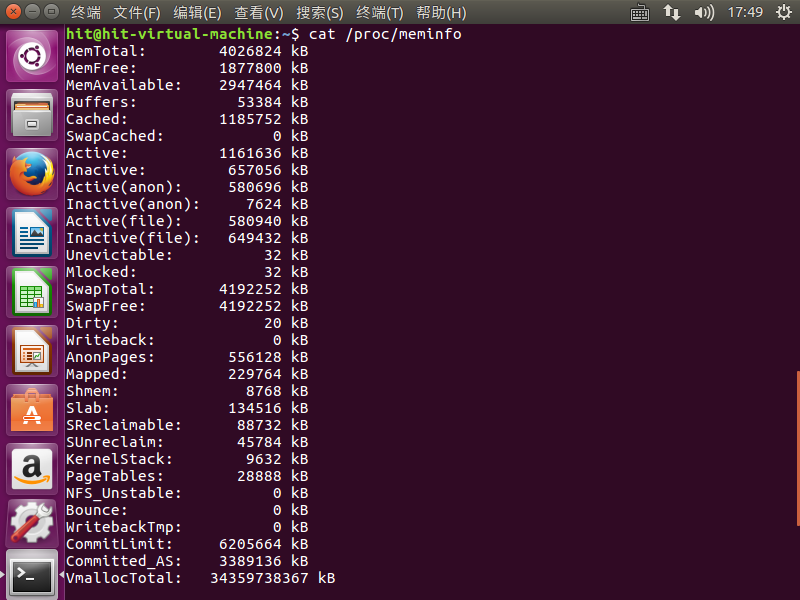
\includegraphics[width=0.7\linewidth]{figures/Lin-Mem}
		\label{fig:lin-mem}
	\end{minipage}
	\begin{minipage}[c]{0.5\linewidth}
		\centering
		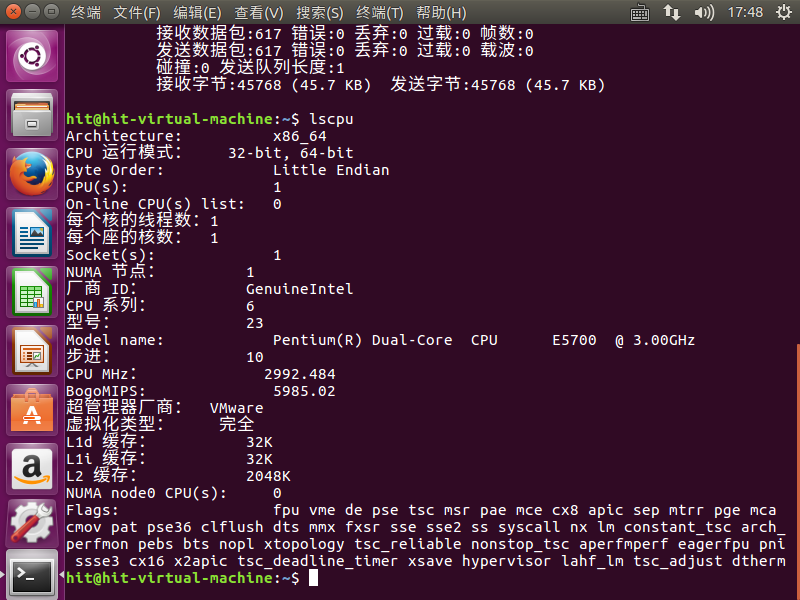
\includegraphics[width=0.7\linewidth]{figures/Lin-Cpu}
		\label{fig:lin-cpu}
	\end{minipage}
	\caption{Linux下计算机硬件详细信息}
\end{figure}

\subsection{任务管理与资源监视(2分)}
写出Linux下的PID最小的两个任务的PID、名称(Command)。

\begin{tabular}{|c|c|}
	\hline 
	PID & Command \\ 
	\hline 
	1 & /sbin/init \\ 
	\hline 
	189 & /usr/lib/systemd/systemd-journald \\ 
	\hline 
\end{tabular} 

\subsection{共享目录的文件系统信息(3分)}
写出Linux下的hitics共享目录对应的文件系统的基本信息:

\begin{itemize}
	\item 名称:\dlmu[3cm]{hitics}
	\item 容量:\dlmu[3cm]{10.0kb}
	\item 挂载点:\dlmu[3cm]{/mnt/hgfs/hitics}
\end{itemize}

\subsection{LINUX下网络系统信息(2分)}

\begin{itemize}
	\item 写出本虚拟机的IPv4地址:\dlmu[3cm]{192.168.75.129}
	\item Mac地址:\dlmu[3cm]{00:0c:29:a2:9d:7d}
\end{itemize}

\begin{figure}[H]
	\centering
	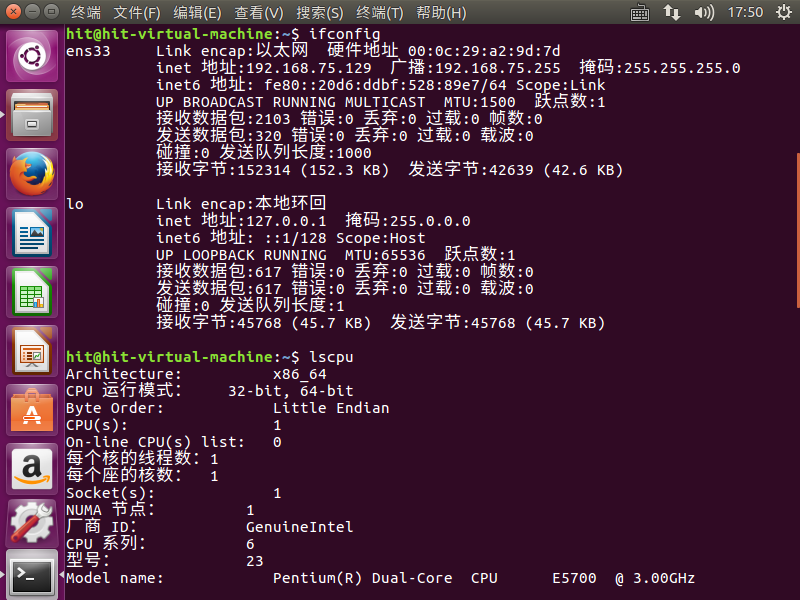
\includegraphics[width=0.7\linewidth]{figures/Lin-Net}
	\caption{Linux下网络系统信息}
	\label{fig:lin-net}
\end{figure}
